\chapter{Numerical experiments and simulation results}


\begin{figure}[!htb] %Change this to [p] maybe ?
    \centering
    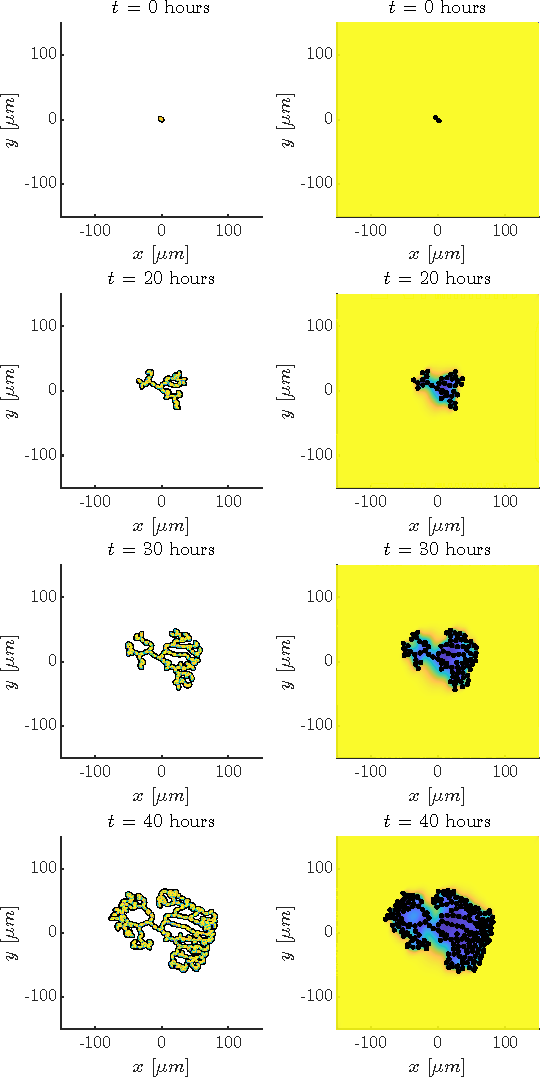
\includegraphics[width= 0.7\textwidth]{
        chapter3/figures/t_all_L1_0o10_L2_5o00_L3_5o00_L4_0o50_L5_1o00_L6_3o00_L7_0o50.pdf}
    \caption{A cell colony with parameter values given by
             $\lambda_1 = 0.1$,  
             $\lambda_2 = 5.0$, 
             $\lambda_3 = 5.0$, 
             $\lambda_4 = 0.5$, 
             $\lambda_5 = 1.0$, 
             $\lambda_6 = 3.0$, 
             $\lambda_7 = 0.5$. 
             On the left we have the biomass field, the nutrient field is on the right.}
    \label{fig: sdsd}
\end{figure}

\begin{figure}[!htb] %Change this to [p] maybe ?
    \centering
    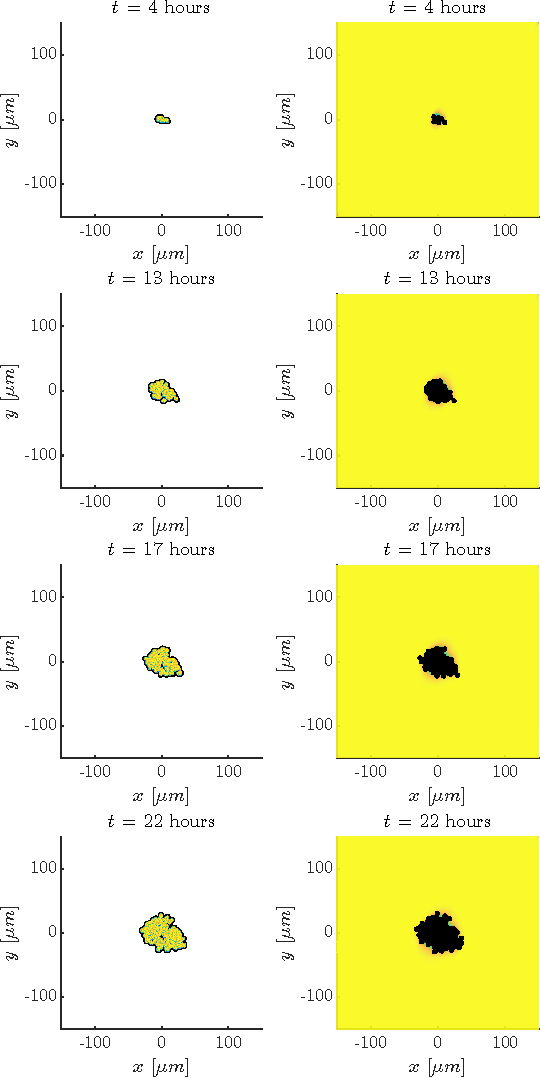
\includegraphics[width= 0.7\textwidth]{
        chapter3/figures/t_all_L1_0o10_L2_5o00_L3_5o00_L4_0o50_L5_0o10_L6_0o70_L7_0o73.pdf}
    \caption{A cell colony with parameter values given by
             $\lambda_1 = 0.1$,  
             $\lambda_2 = 5.0$, 
             $\lambda_3 = 5.0$, 
             $\lambda_4 = 0.5$, 
             $\lambda_5 = 0.1$, 
             $\lambda_6 = 0.7$, 
             $\lambda_7 = 0.73$. 
             On the left we have the biomass field, the nutrient field is on the right. 
             The aspect ratio is $\lambda_7 = 5.5/7.5 = 0.73$.}
    \label{fig: sdsd}
\end{figure}

\begin{figure}[!htb] 
    \centering
    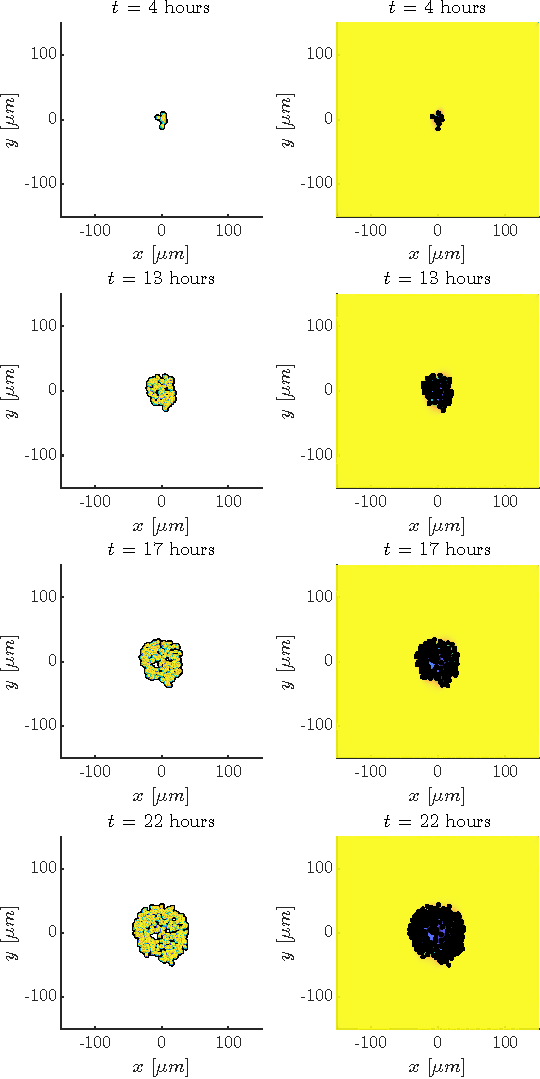
\includegraphics[width= 0.7\textwidth]{
        chapter3/figures/t_all_L1_0o10_L2_5o00_L3_5o00_L4_0o50_L5_1o20_L6_0o70_L7_0o60.pdf}
    \caption{A cell colony with parameter values given by
             $\lambda_1 = 0.1$,  
             $\lambda_2 = 5.0$, 
             $\lambda_3 = 5.0$, 
             $\lambda_4 = 0.5$, 
             $\lambda_5 = 1.2$, 
             $\lambda_6 = 0.7$, 
             $\lambda_7 = 0.6$. 
             Biomass on left and nutrient field on the right.}
    \label{fig: sdsd}
\end{figure}

\begin{figure}[!htb] %Change this to [p] maybe ?
    \centering
    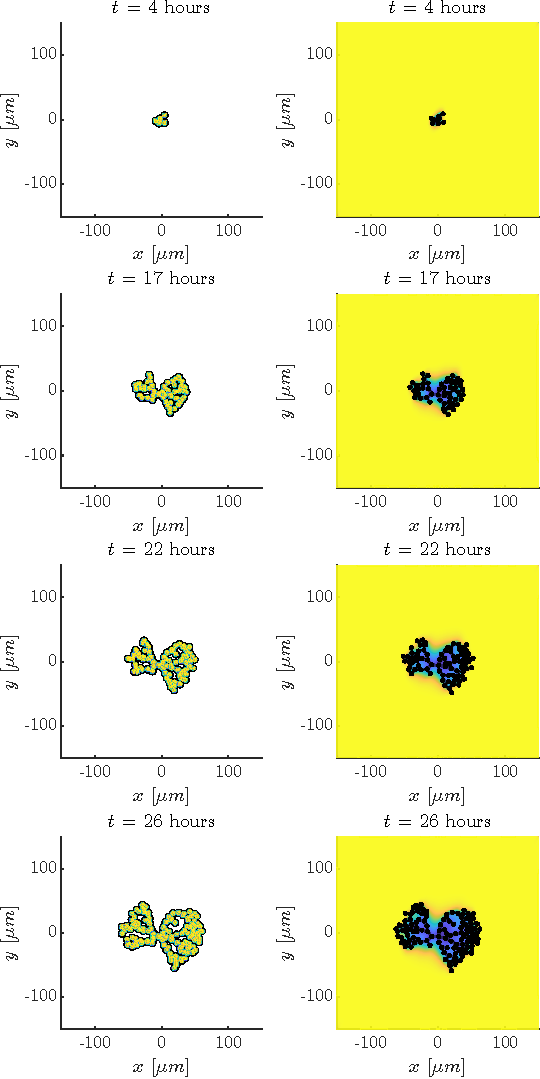
\includegraphics[width= 0.7\textwidth]{
        chapter3/figures/t_all_L1_0o10_L2_5o00_L3_5o00_L4_0o50_L5_1o60_L6_0o90_L7_0o95.pdf}
    \caption{A cell colony with parameter values given by
             $\lambda_1 = 0.1$,  
             $\lambda_2 = 5.0$, 
             $\lambda_3 = 5.0$, 
             $\lambda_4 = 0.5$, 
             $\lambda_5 = 1.6$, 
             $\lambda_6 = 0.9$, 
             $\lambda_7 = 0.95$. 
             Biomass on left and nutrient field on the right.}
    \label{fig: sdsd}
\end{figure}

\begin{figure}[!htb] %Change this to [p] maybe ?
    \centering
    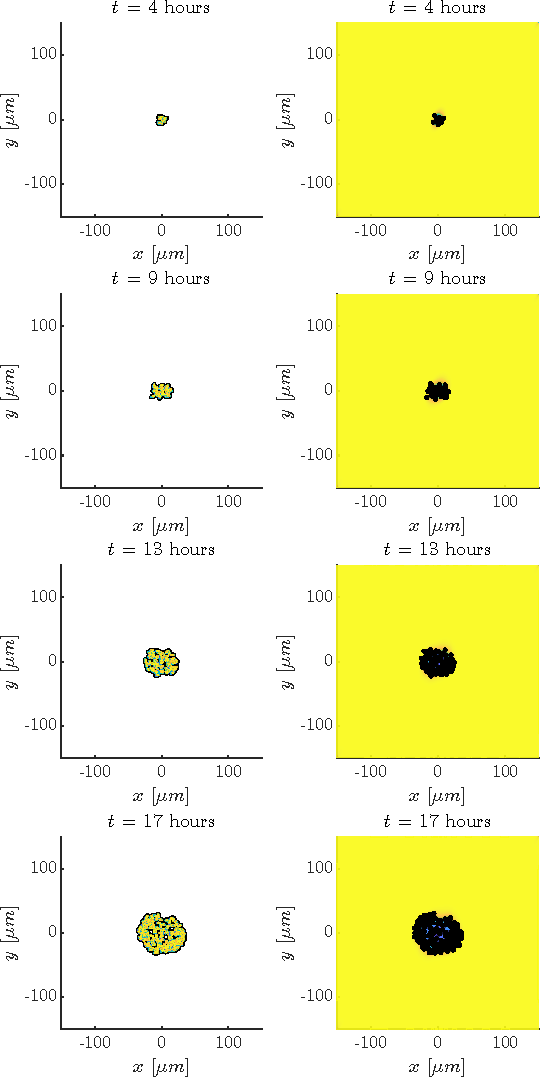
\includegraphics[width= 0.7\textwidth]{
        chapter3/figures/t_all_L1_0o10_L2_5o00_L3_5o00_L4_0o50_L5_1o60_L6_0o70_L7_0o50.pdf}
    \caption{A cell colony with parameter values given by
             $\lambda_1 = 0.1$,  
             $\lambda_2 = 5.0$, 
             $\lambda_3 = 5.0$, 
             $\lambda_4 = 0.5$, 
             $\lambda_5 = 1.6$, 
             $\lambda_6 = 0.7$, 
             $\lambda_7 = 0.5$. 
             Biomass on left and nutrient field on the right.}
    \label{fig: sdsd}
\end{figure}

\begin{figure}[!htb]
    \centering
    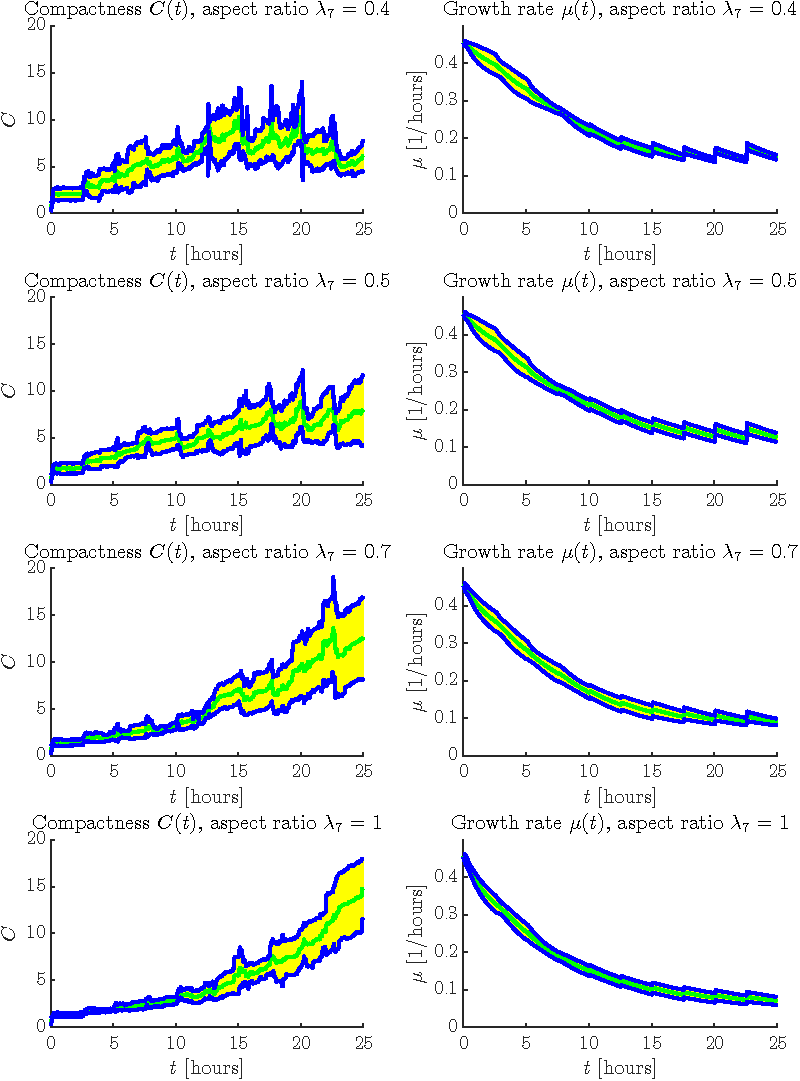
\includegraphics[width= \textwidth]{
        chapter3/figures/Comp_all_ar_EnsembleSize_6o0_L1_0o10_L2_5o00_L3_5o00_L4_0o50_L5_1o00_L6_1o00_L7_0o40.pdf}
    \caption{The colony compactness and growth rate for 
             $\lambda_1 = 0.1$,  
             $\lambda_2 = 5.0$, 
             $\lambda_3 = 5.0$, 
             $\lambda_4 = 0.5$, 
             $\lambda_5 = 1.0$, 
             $\lambda_6 = 1.0$, 
             $\lambda_7$ variable and an ensemble size of $6$.}
    \label{fig: sdsd}
\end{figure}

\begin{figure}[!htb] %Change this to [p] maybe ?
    \centering
    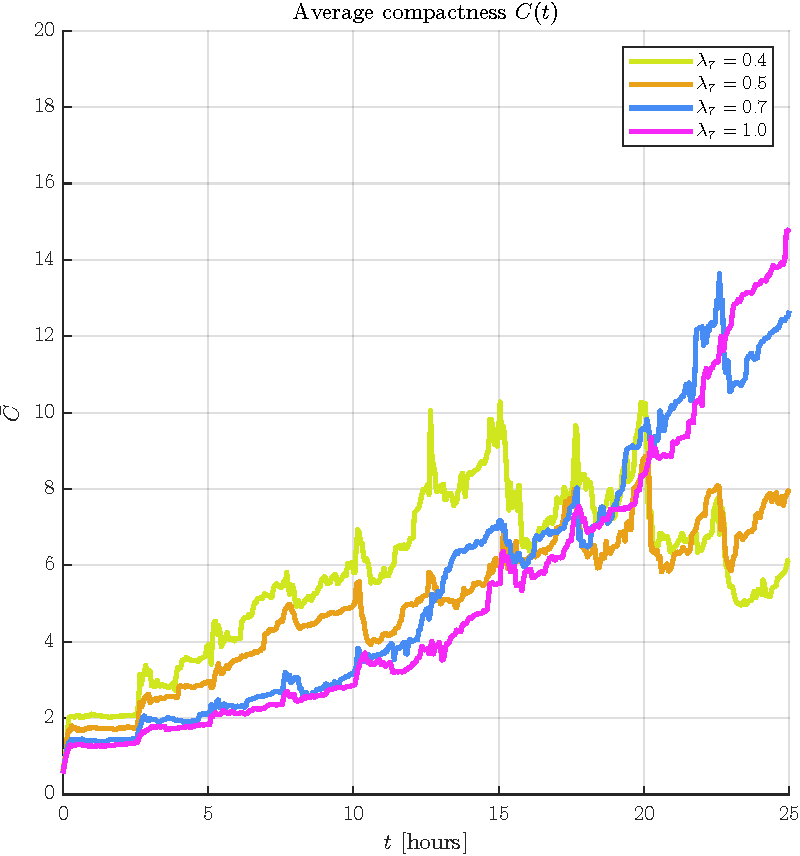
\includegraphics[width= \textwidth]{
        chapter3/figures/Comp_average_actness_EnsembleSize_6o0_L1_0o10_L2_5o00_L3_5o00_L4_0o50_L5_1o00_L6_1o00_L7_0o40.pdf}
    \caption{The average colony compactness for
             $\lambda_1 = 0.1$,  
             $\lambda_2 = 5.0$, 
             $\lambda_3 = 5.0$, 
             $\lambda_4 = 0.5$, 
             $\lambda_5 = 1.0$, 
             $\lambda_6 = 1.0$, 
             $\lambda_7 = 0.4, 0.5, 0.7, 1.0$ and an ensemble size of $6$.}
    \label{fig: sdsd}
\end{figure}

\begin{figure}[!htb] %Change this to [p] maybe ?
    \centering
    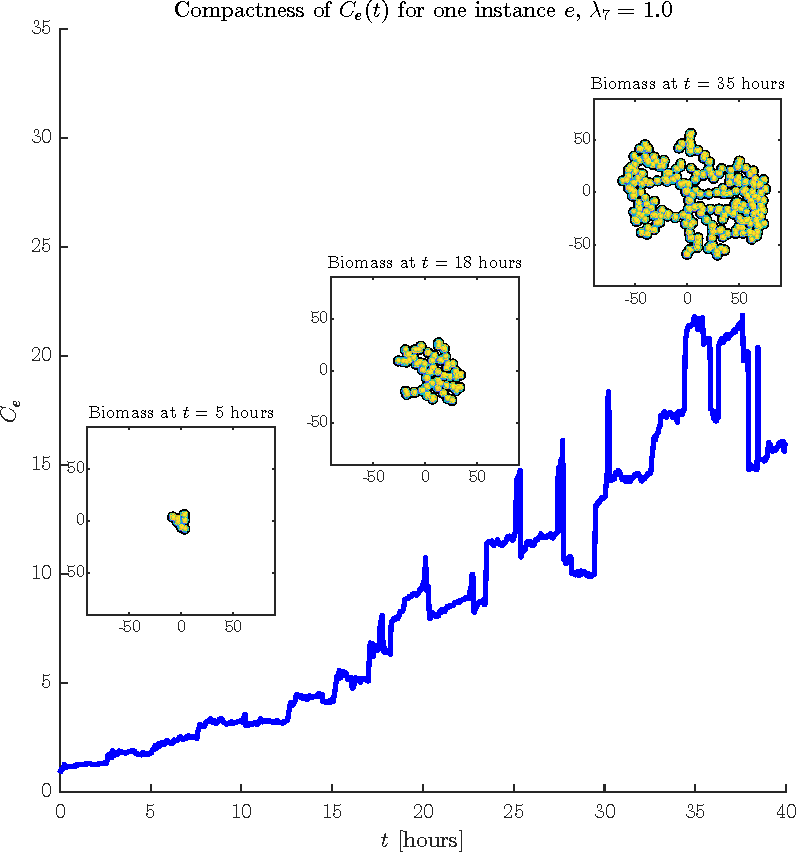
\includegraphics[width= \textwidth]{
        chapter3/figures/Inset_L1_0o10_L2_5o00_L3_5o00_L4_0o50_L5_1o00_L6_1o00_L7_1o00.pdf}
    \caption{Compactness for ensemble instance $e = 1$ and 
             $\lambda_1 = 0.1$,  
             $\lambda_2 = 5.0$, 
             $\lambda_3 = 5.0$, 
             $\lambda_4 = 0.5$, 
             $\lambda_5 = 1.0$, 
             $\lambda_6 = 1.0$, 
             $\lambda_7 = 1.0$. The inset plots show the biomass at three times for comparison 
             with compactness.}
    \label{fig: sdsd}
\end{figure}

\begin{figure}[!htb] %Change this to [p] maybe ?
    \centering
    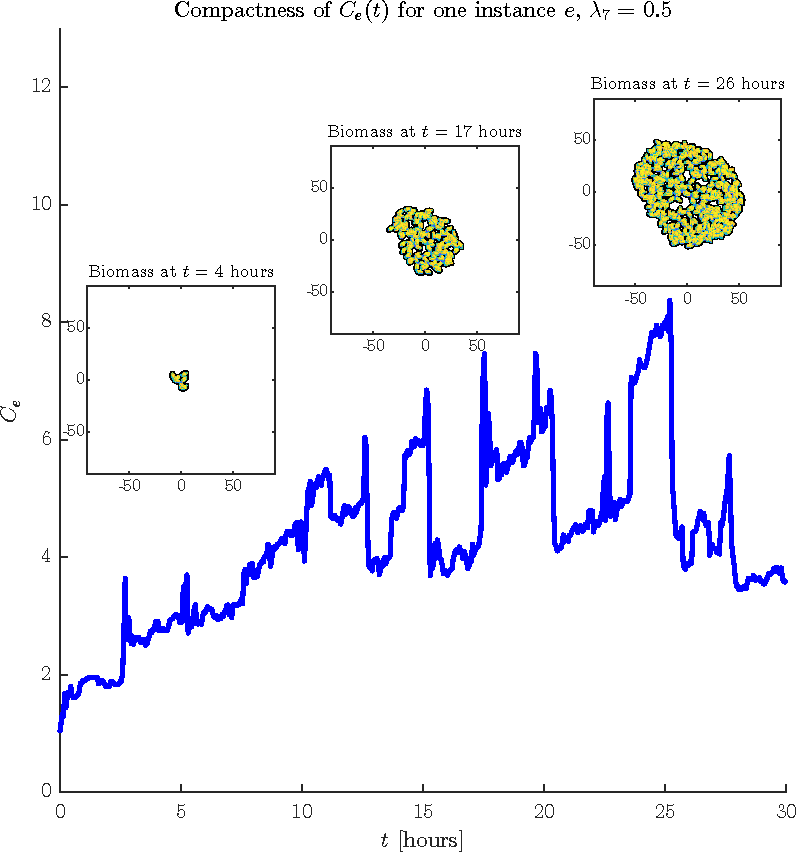
\includegraphics[width= \textwidth]{
        chapter3/figures/Inset_L1_0o10_L2_5o00_L3_5o00_L4_0o50_L5_1o00_L6_1o00_L7_0o50.pdf}
    \caption{Compactness for ensemble instance $e = 1$ and 
             $\lambda_1 = 0.1$,  
             $\lambda_2 = 5.0$, 
             $\lambda_3 = 5.0$, 
             $\lambda_4 = 0.5$, 
             $\lambda_5 = 1.0$, 
             $\lambda_6 = 1.0$, 
             $\lambda_7 = 0.5$. The inset plots show the biomass at three times for comparison 
             with compactness.}
    \label{fig: sdsd}
\end{figure}


\begin{figure}[!htb] %Change this to [p] maybe ?
    \centering
    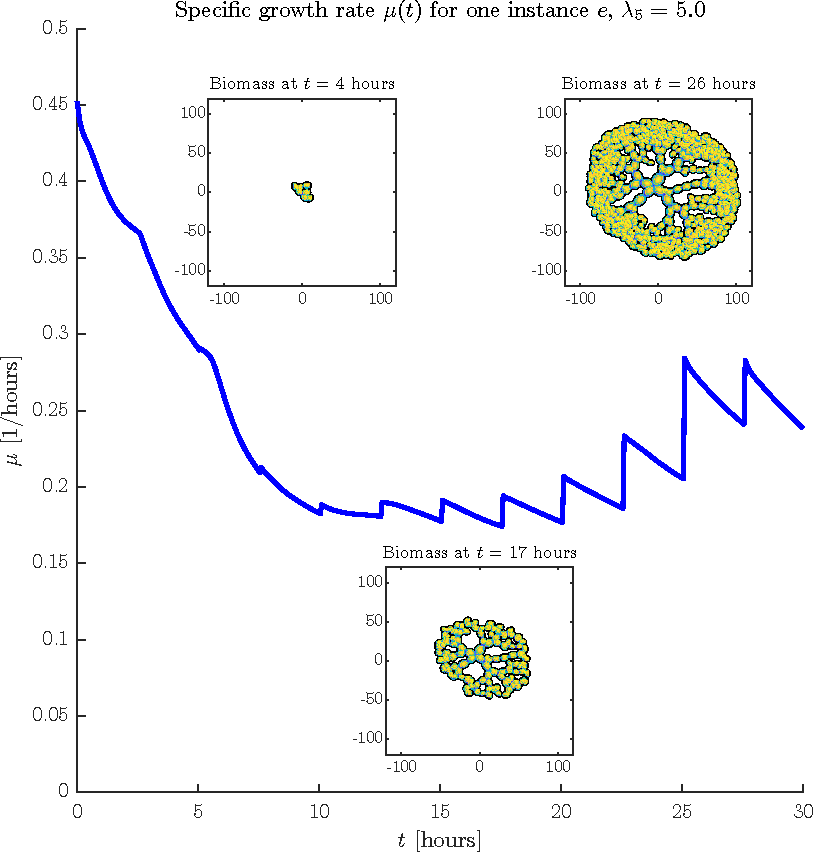
\includegraphics[width= \textwidth]{
        chapter3/figures/Inset_L1_0o10_L2_5o00_L3_5o00_L4_0o50_L5_5o00_L6_1o00_L7_0o70.pdf}
    \caption{Specific growth rate $\mu(t)$ for ensemble instance $e = 1$ and 
             $\lambda_1 = 0.1$,  
             $\lambda_2 = 5.0$, 
             $\lambda_3 = 5.0$, 
             $\lambda_4 = 0.5$, 
             $\lambda_5 = 5.0$, 
             $\lambda_6 = 1.0$, 
             $\lambda_7 = 0.7$.}
    \label{fig: sdsd}
\end{figure}

\begin{figure}[!htb] %Change this to [p] maybe ?
    \centering
    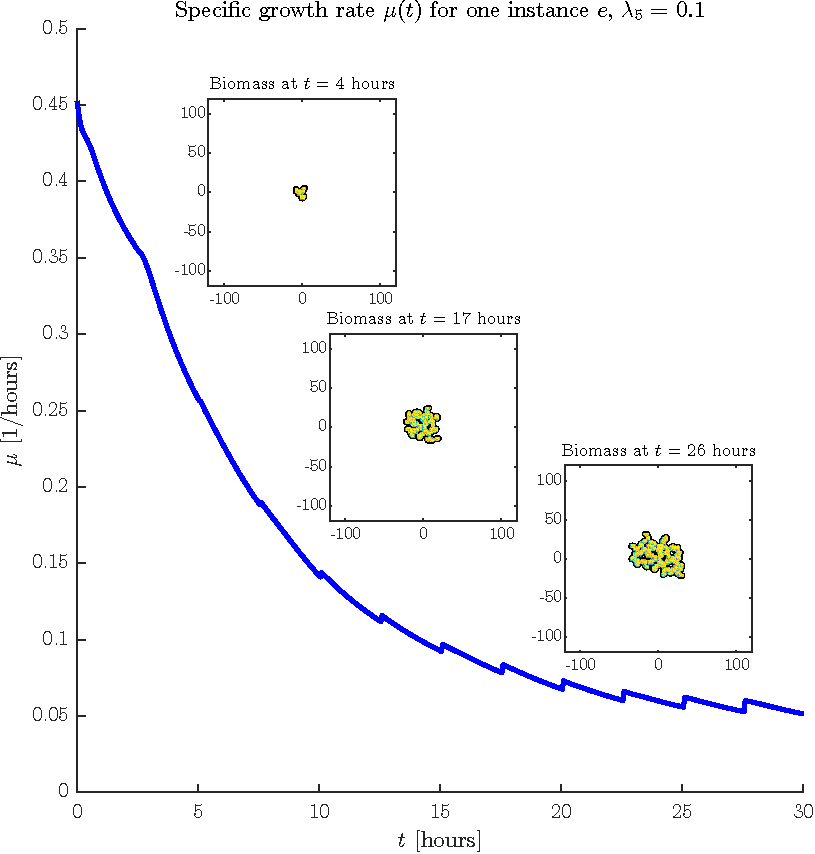
\includegraphics[width= \textwidth]{
        chapter3/figures/Inset_L1_0o10_L2_5o00_L3_5o00_L4_0o50_L5_0o10_L6_1o00_L7_0o70.pdf}
    \caption{Specific growth rate $\mu(t)$ for ensemble instance $e = 1$ and 
             $\lambda_1 = 0.1$,  
             $\lambda_2 = 5.0$, 
             $\lambda_3 = 5.0$, 
             $\lambda_4 = 0.5$, 
             $\lambda_5 = 0.1$, 
             $\lambda_6 = 1.0$, 
             $\lambda_7 = 0.7$.}
    \label{fig: sdsd}
\end{figure}

\begin{figure}[!htb] %Change this to [p] maybe ?
    \centering
    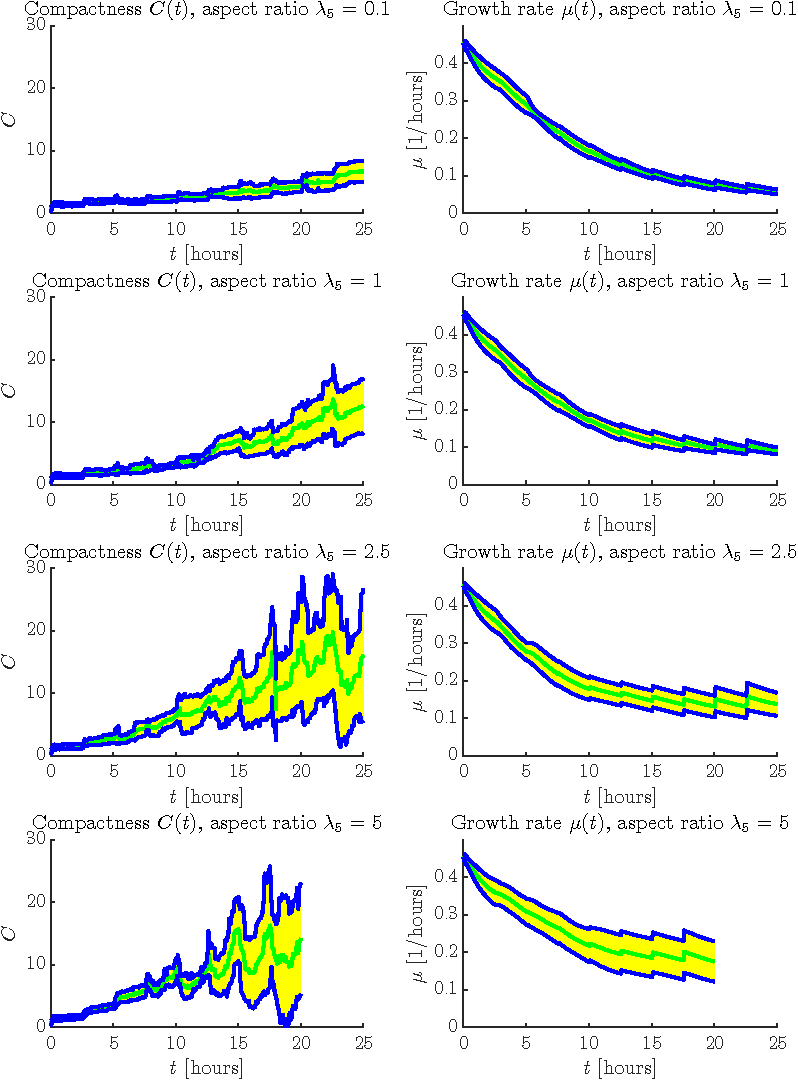
\includegraphics[width= \textwidth]{
        chapter3/figures/Comp_all_ar_EnsembleSize_6o0_L1_0o10_L2_5o00_L3_5o00_L4_0o50_L5_0o10_L6_1o00_L7_0o70.pdf}
    \caption{Compactness $C(t)$ and specific growth rate $\mu(t)$ for 
             $\lambda_1 = 0.1$,  
             $\lambda_2 = 5.0$, 
             $\lambda_3 = 5.0$, 
             $\lambda_4 = 0.5$, 
             $\lambda_5 = 0.1, 1.0, 2.5, 5.0$, 
             $\lambda_6 = 1.0$, 
             $\lambda_7 = 0.7$, and an ensemble of size $6$. Note that the bottom panels 
             could only be simulated to $t = 20$ hours due to GPU out-of-memory issues.}
    \label{fig: sdsd}
\end{figure}

\begin{figure}[!htb] %Change this to [p] maybe ?
    \centering
    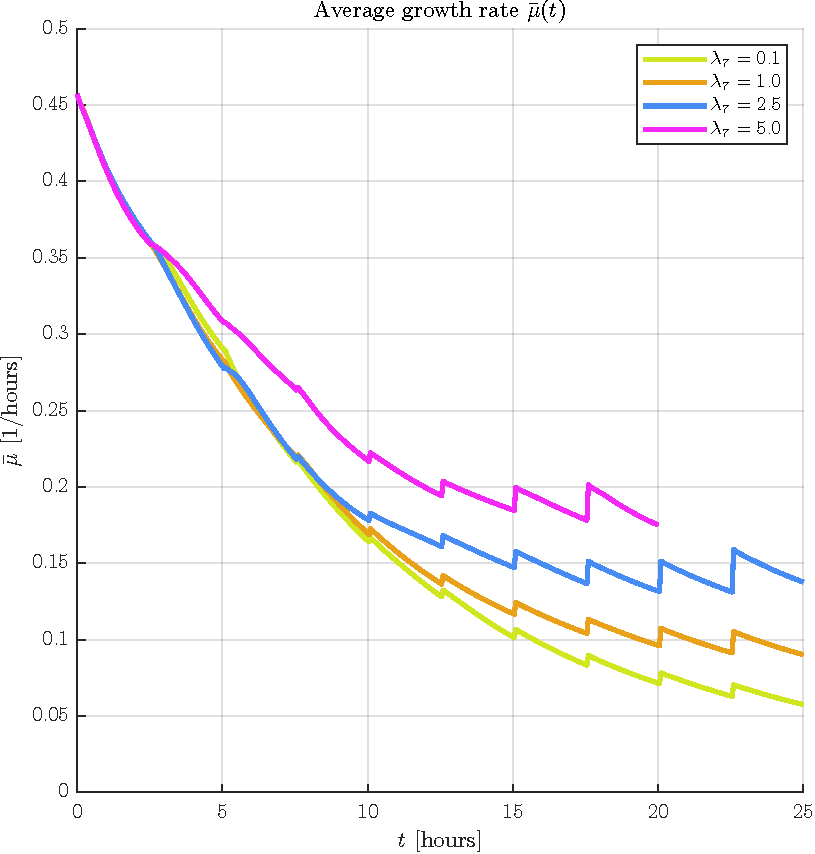
\includegraphics[width= \textwidth]{
        chapter3/figures/Average_mu_EnsembleSize_6o0_L1_0o10_L2_5o00_L3_5o00_L4_0o50_L5_0o10_L6_1o00_L7_0o70.pdf}
    \caption{Average growth rate $\mu(t)$ for 
             $\lambda_1 = 0.1$,  
             $\lambda_2 = 5.0$, 
             $\lambda_3 = 5.0$, 
             $\lambda_4 = 0.5$, 
             $\lambda_5 = 0.1, 1.0, 2.5, 5.0$, 
             $\lambda_6 = 1.0$, 
             $\lambda_7 = 0.7$, and an ensemble of size $6$. Note the plot 
             for $\lambda_5 = 5.0$ could not be completed on the aviliable hardware
             due to GPU out-of-memory.}
    \label{fig: sdsd}
\end{figure}

